\chapter{系统架构}

基于可重构硬件的智能网卡。需要讨论以智能网卡为中心的服务器软硬件架构。基本思想:可编程网卡是服务器与外界之间通信的“网关”,也是服务器内硬件设备、虚拟机间通信的“枢纽”,把 hypervisor 和 OS kernel 中需要高性能的数据平面卸载到可编程网卡。

画一个数据中心架构图,包括存储、网关等节点,计算节点(包括 hypervisor 和客户虚拟机)。


\begin{figure}[htbp]
	\centering
	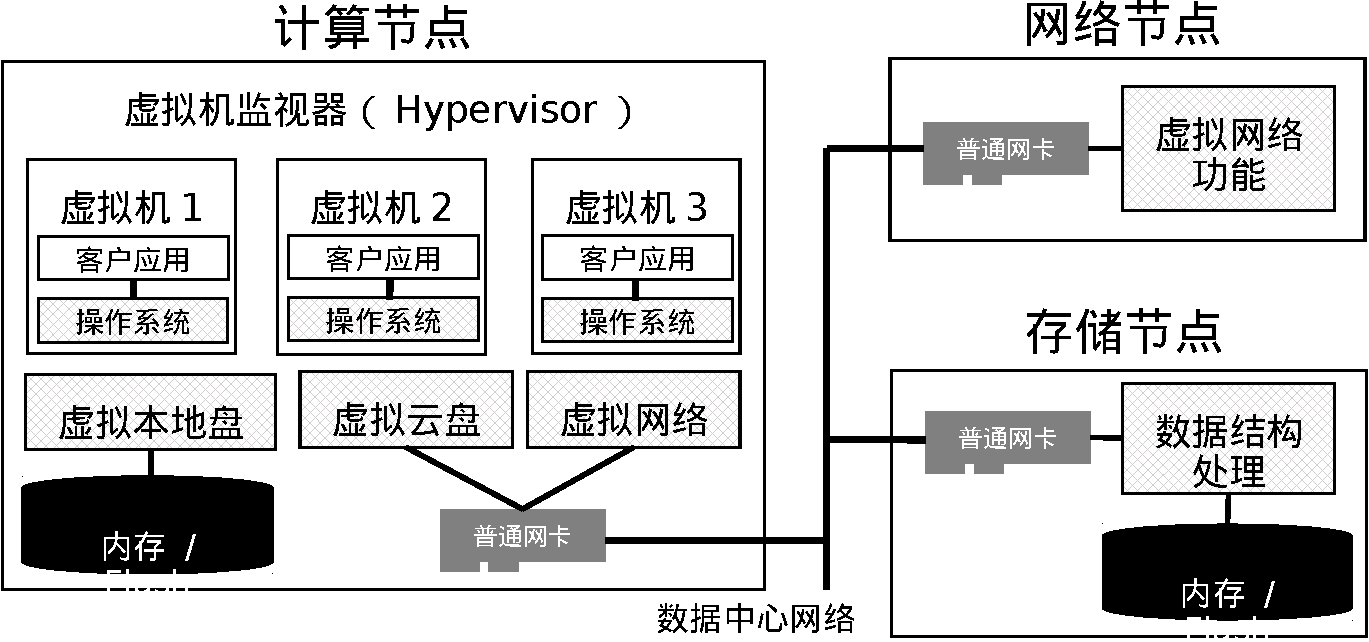
\includegraphics[width=0.8\textwidth]{figures/virt_arch.pdf}
	\caption{回顾:基于软件的虚拟化数据中心架构。}
	\label{arch:fig:virt-architecture}
\end{figure}


\begin{figure}[htbp]
	\centering
	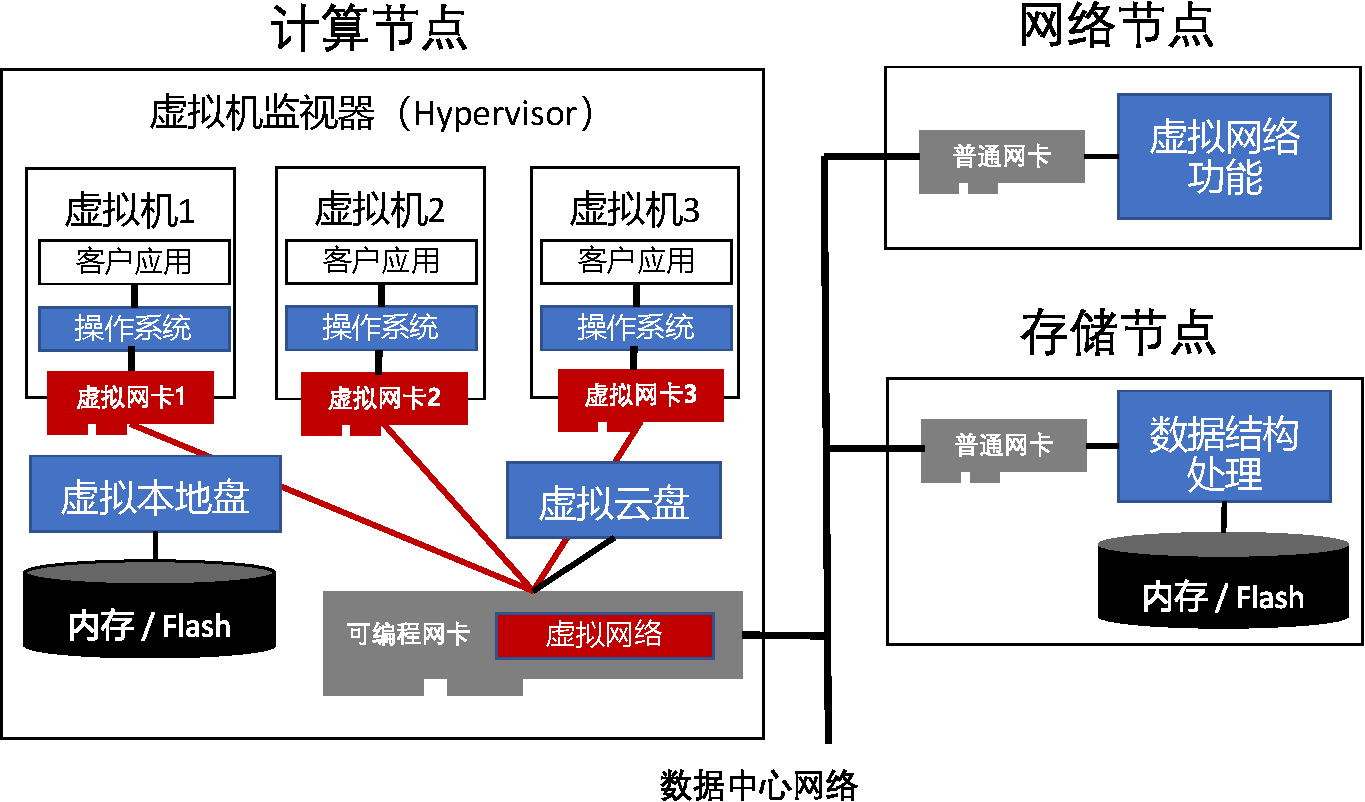
\includegraphics[width=0.8\textwidth]{figures/virtual_network.pdf}
	\caption{用可编程网卡加速虚拟网络后的架构。}
	\label{arch:fig:virtual-network}
\end{figure}

\begin{figure}[htbp]
	\centering
	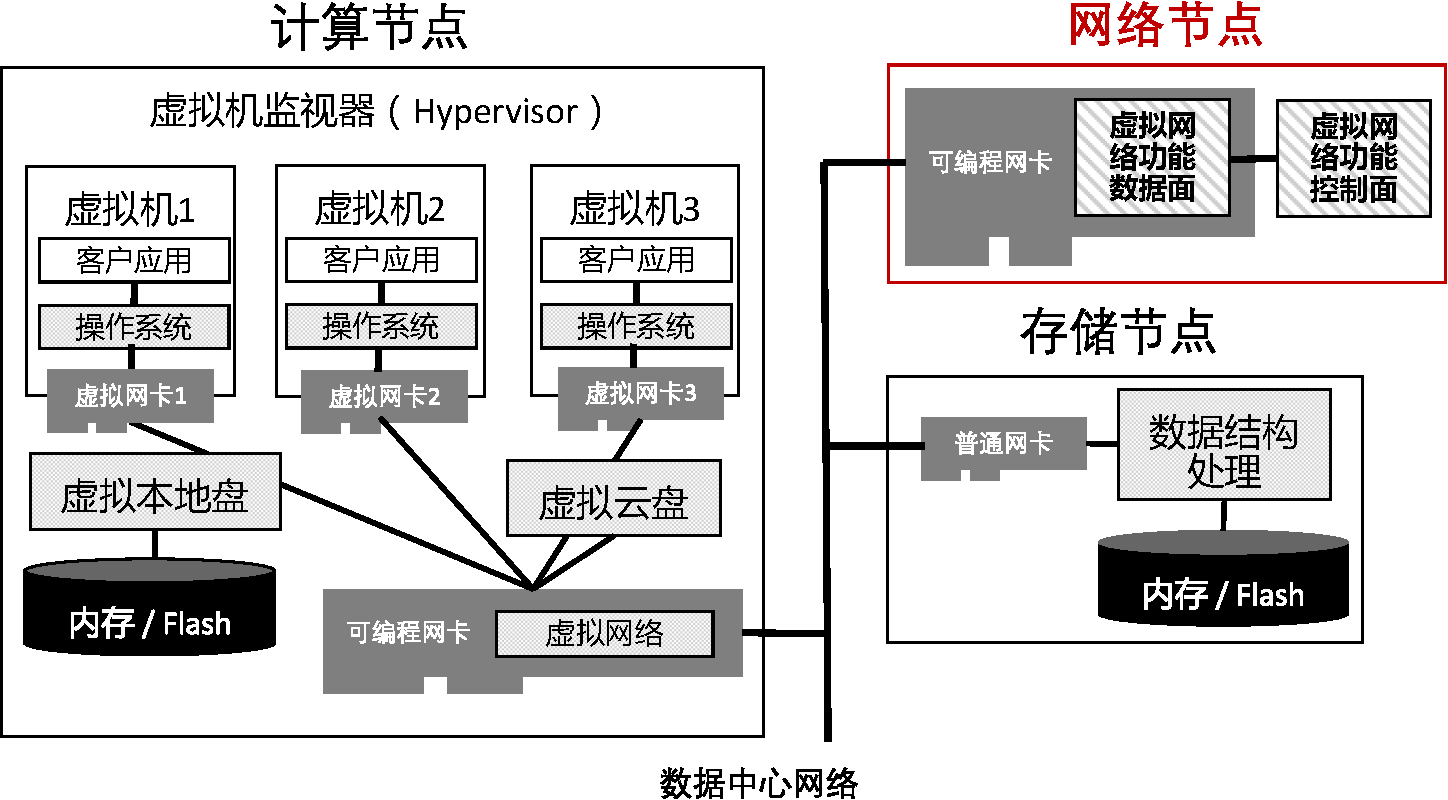
\includegraphics[width=0.8\textwidth]{figures/NFV_accel.pdf}
	\caption{用可编程网卡加速网络功能后的架构。}
	\label{arch:fig:network-function}
\end{figure}


\begin{figure}[htbp]
	\centering
	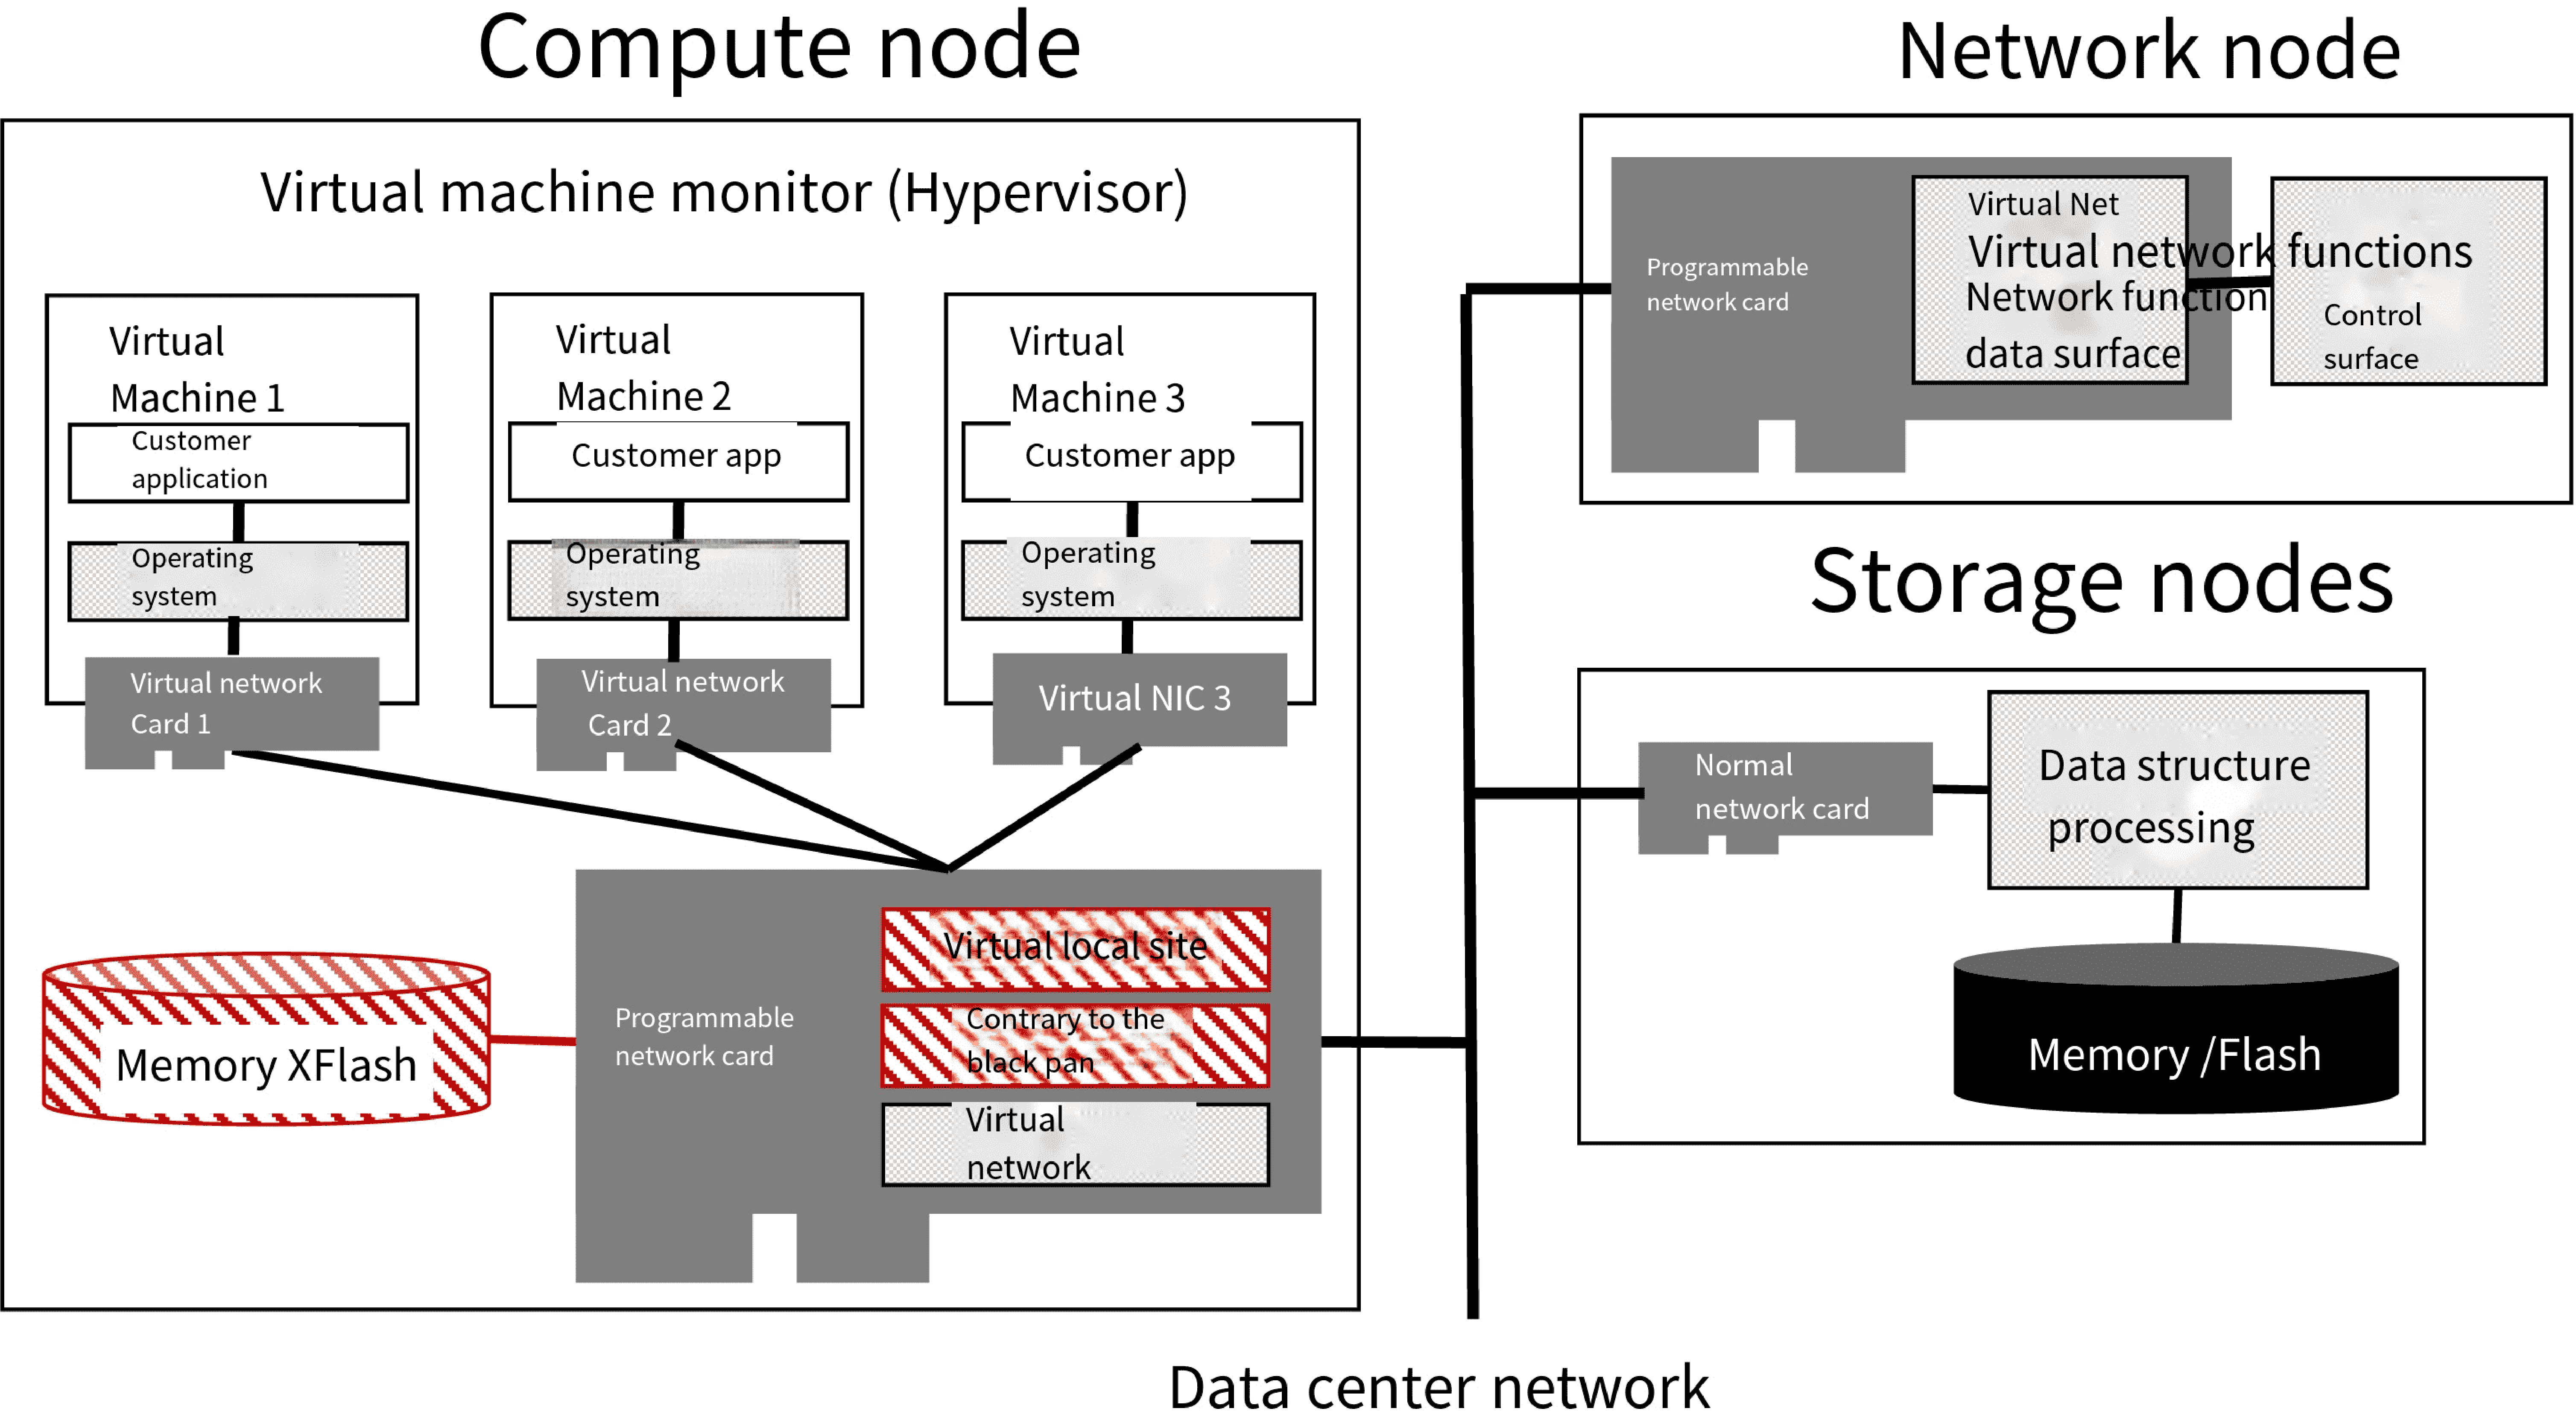
\includegraphics[width=0.8\textwidth]{figures/virt_storage.pdf}
	\caption{用可编程网卡加速本地存储和云存储后的架构。}
	\label{arch:fig:virt-storage}
\end{figure}

\begin{figure}[htbp]
	\centering
	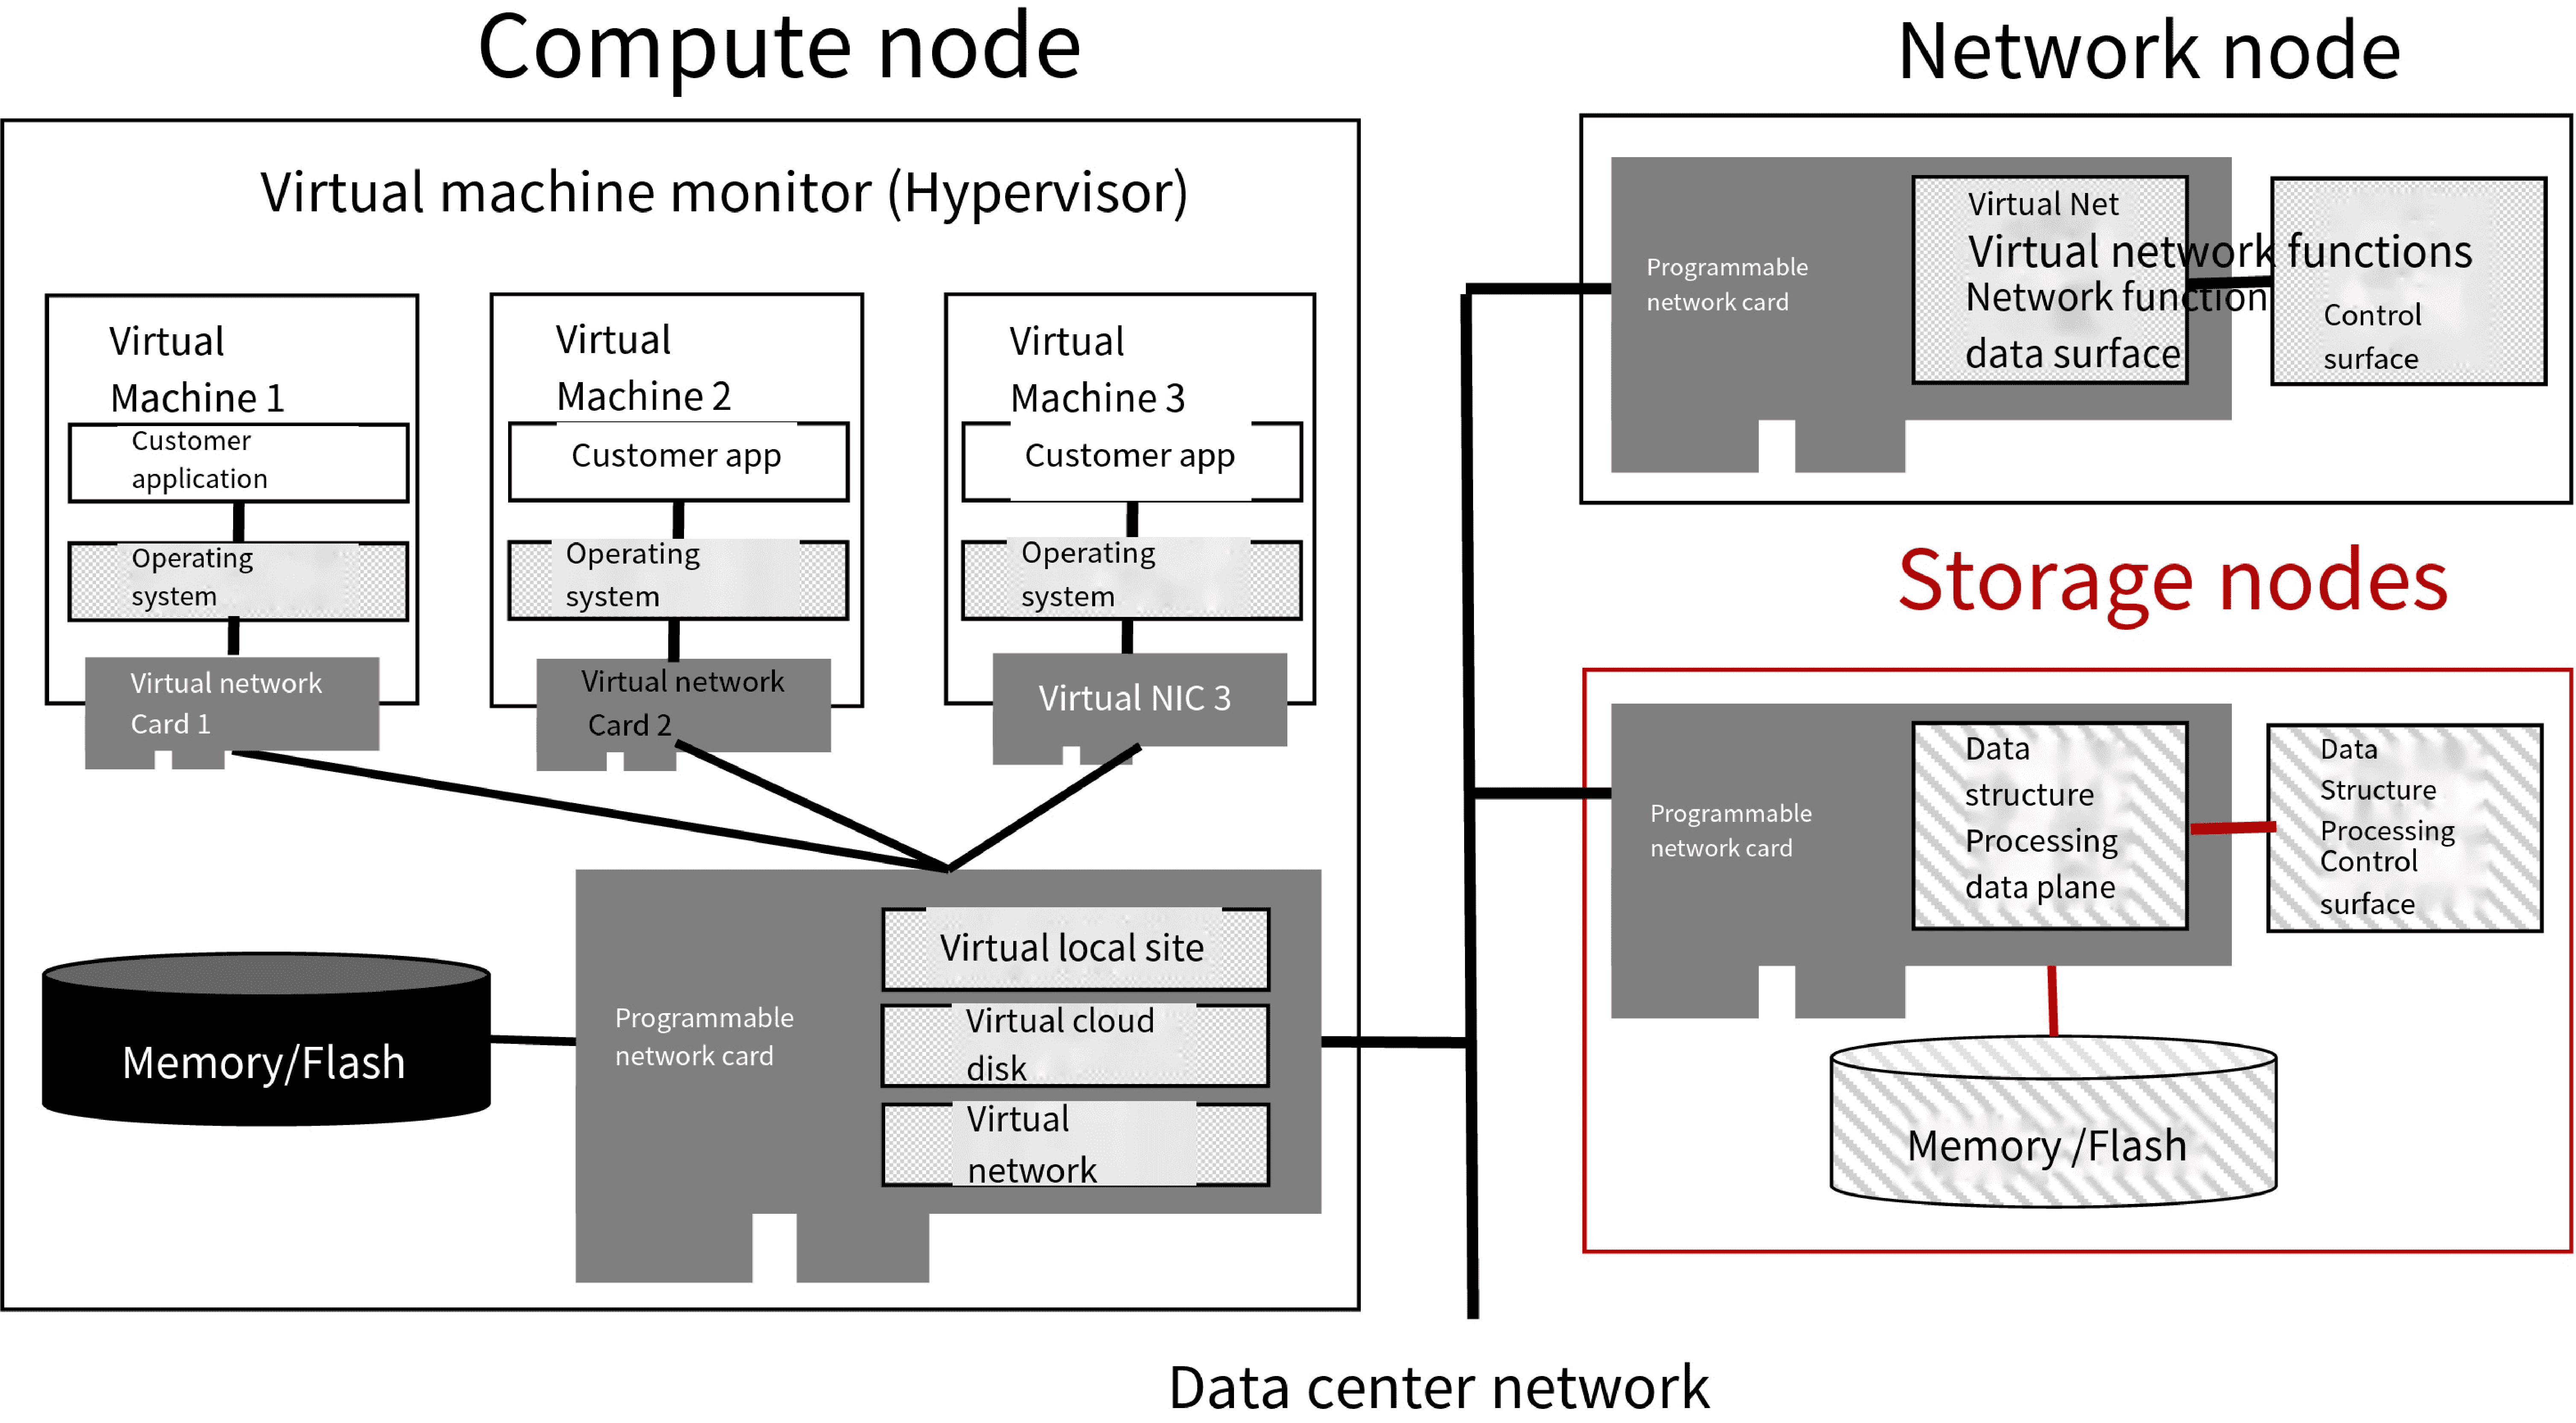
\includegraphics[width=0.8\textwidth]{figures/data_structure_accel.pdf}
	\caption{用可编程网卡加速数据结构处理后的架构。}
	\label{arch:fig:data-structure-accel}
\end{figure}


\begin{figure}[htbp]
	\centering
	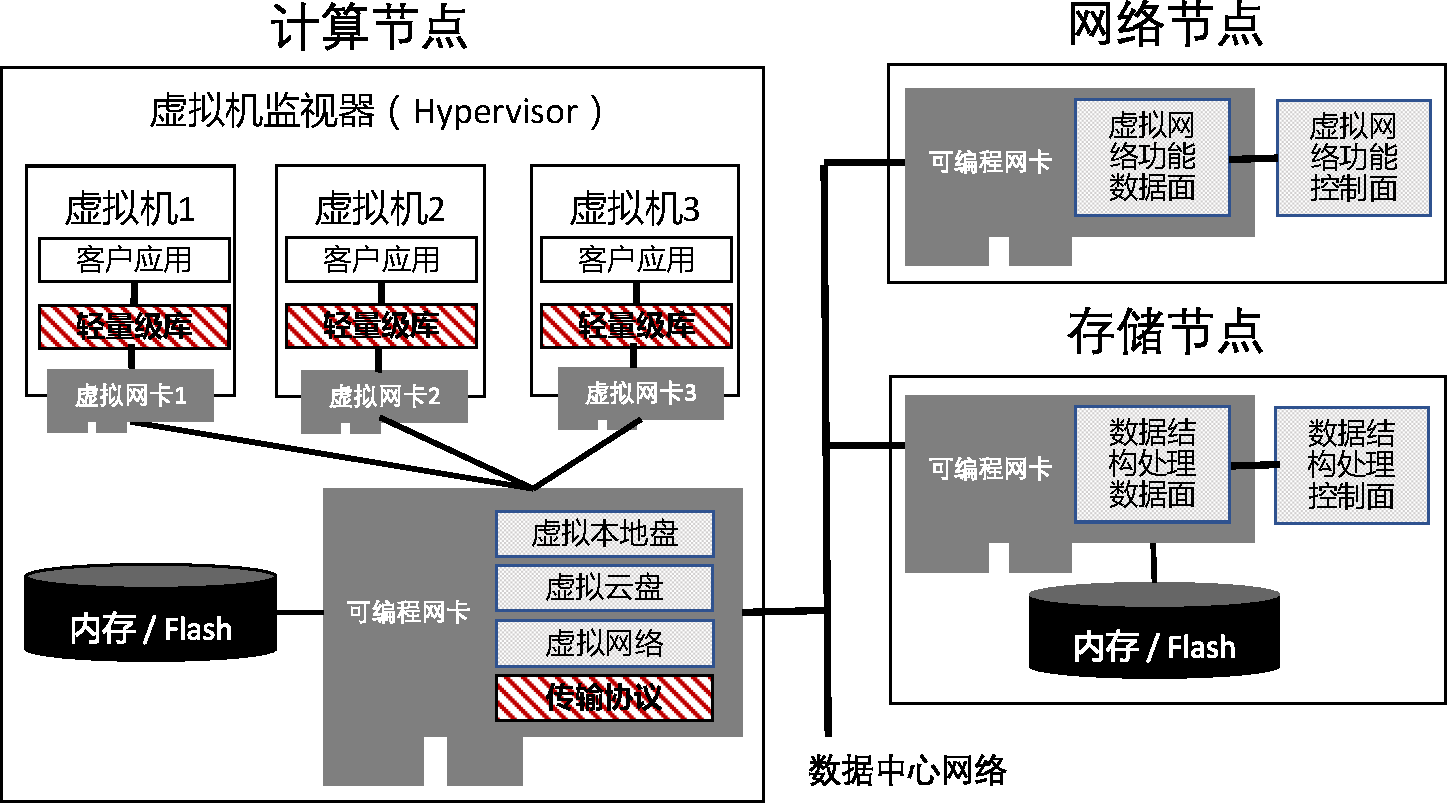
\includegraphics[width=0.8\textwidth]{figures/os_primitives_accel.pdf}
	\caption{用可编程网卡加速操作系统通信原语后的架构。}
	\label{arch:fig:os-primitives-accel}
\end{figure}


\begin{figure}[htbp]
	\centering
	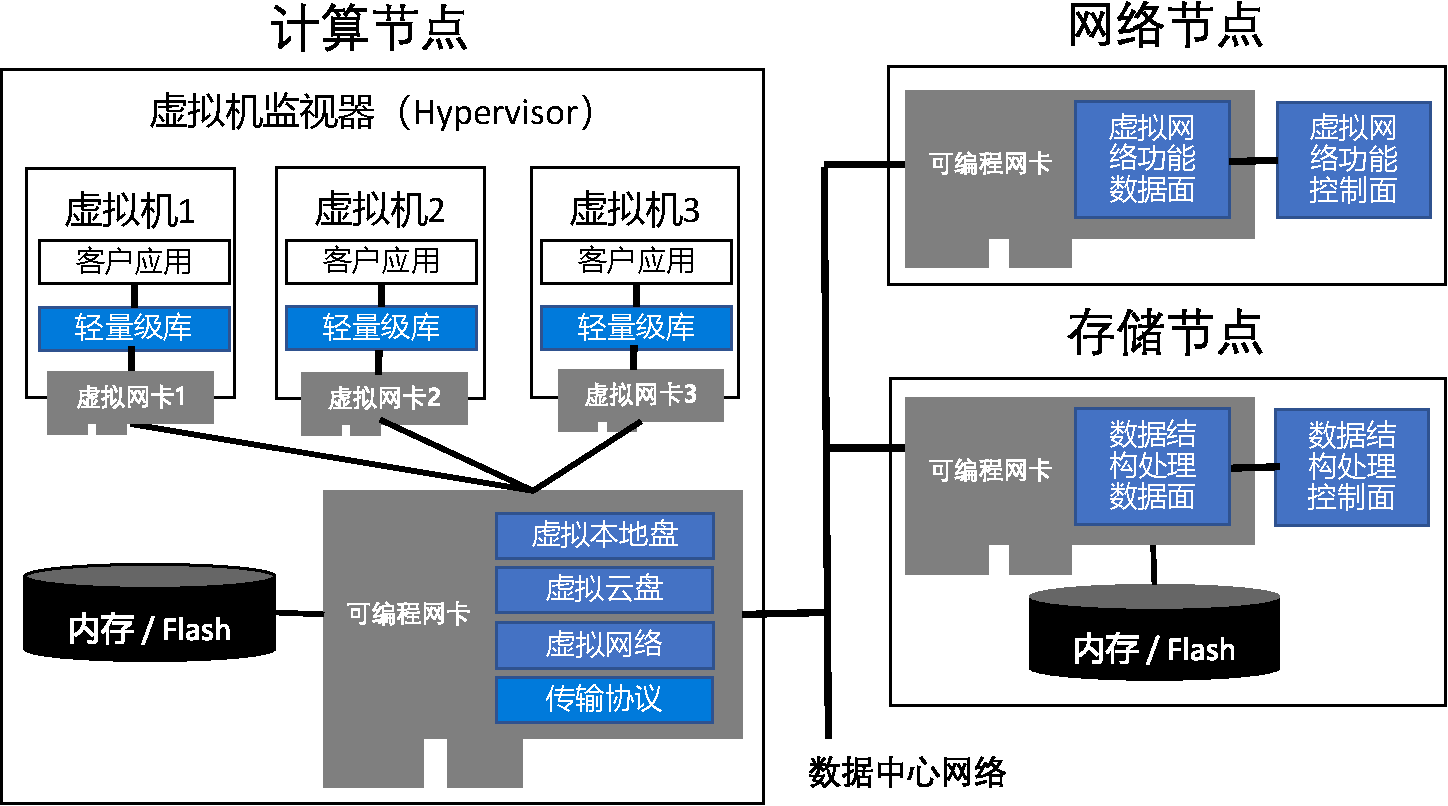
\includegraphics[width=0.8\textwidth]{figures/accel_arch.pdf}
	\caption{基于可编程网卡的数据中心系统总体架构。}
	\label{arch:fig:accel-arch}
\end{figure}



\begin{figure}[htbp]
	\centering
	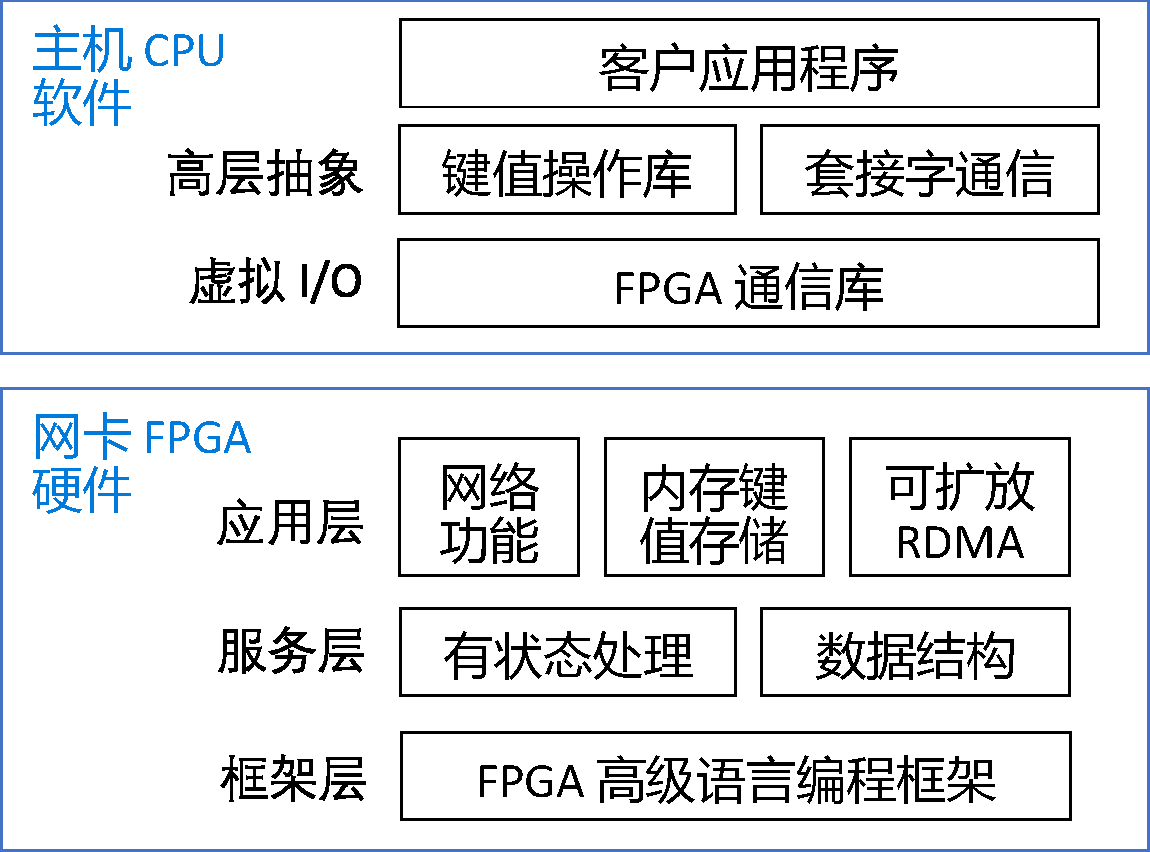
\includegraphics[width=0.6\textwidth]{figures/sw_hw_codesign.pdf}
	\caption{软硬件协同设计的可编程网卡架构。}
	\label{arch:fig:sw-hw-codesign}
\end{figure}

\section{计算节点}

位置:计算节点(客户虚拟机所在的服务器)。

\subsection{虚拟化}

虚拟机监控器(hypervisor):硬件的一虚多、多虚一。

\subsubsection{一虚多}

可编程网卡把主机内的硬件资源虚拟化成多个逻辑资源,实现外部机器和本地虚拟机的多路复用(ClickNP 硬件网卡虚拟化为多个租户的 VPC,SocksDirect 容器网络,即 vSwitch data-plane offload)。

\subsubsection{多虚一}

可编程网卡把数据中心内物理上分散的资源虚拟化成一个逻辑资源(ClickNP VPC 和 SocksDirect 容器网络,KV-Direct 分布式存储的客户端,还可以做 storage 和 memory 的 disaggregation)。

\subsection{高层抽象}

操作系统和共享运行库:高层抽象。

\subsubsection{操作系统原语}

OS kernel 给应用程序提供的高层抽象可以重构为(控制面)协调和管理(仍在内核或用户态 daemon) + (数据面)用户态 library 负责高层抽象 + (数据面)可编程网卡负责多路复用、调度唤醒和可靠传输等低层语义,需要思考数据面上软硬件的接口(SocksDirect)。

\subsubsection{数据结构操作原语}

Key-value 为例。

\section{网络、存储节点}

位置:存储、网关等节点。CPU bypass(控制面数据面分离,数据面 offload,控制面仍在 CPU 上)

\subsection{网络功能卸载}

直接处理网络数据包并直接返回,数据面无需经过 CPU(ClickNP NF offload)。

\subsection{网卡直接访问内存数据结构}

直接访问远程硬件资源,而无需经过远程机器的 CPU (KV-Direct内存数据结构的服务器端,还可以访问闪存(SSD)记录日志后直接返回 ACK,缩短处理延迟)。


\section{可编程网卡}

\subsection{硬件架构}

可编程网卡需要高度灵活性。为什么要 FPGA + CPU + ASIC SoC。回应第二章。

\textbf{图1: 网卡 SoC 结构图}

\subsection{高级语言编程框架}

FPGA 高级语言编程:ClickNP,适合流式处理的模块化 FPGA 高级语言编程

\subsection{基础服务中间件}

有状态处理(stateful processing)、数据结构、可扩放 RDMA

本文使用高级语言编程框架实现基础服务中间件,中间件未来可以硬件化。

\subsection{上层应用}

内存键值存储、持久化键值存储、网络功能